%! TEX TS-program = LuaLaTeX

% Gemini theme
% See: https://rev.cs.uchicago.edu/k4rtik/gemini-uccs
% A fork of https://github.com/anishathalye/gemini

\documentclass[12pt, usenames, dvipsnames]{beamer}

% ====================
% Packages
% ====================

\usepackage[T1]{fontenc}
\usepackage{lmodern}
\usepackage[size=a0, scale=1]{beamerposter}
\usetheme{gemini}
\usecolortheme{stanford}

\usepackage{graphicx}
\usepackage{booktabs}

\usepackage{hyperref}
\usepackage{amsthm}
\usepackage{thmtools}

% For theorems and such
\usepackage{amsmath}
\usepackage{amssymb}
\usepackage{mathtools}

\usepackage{natbib}

\usepackage{xcolor}
\usepackage{algorithm}
\usepackage{algorithmic}
\usepackage{bbm}

% ====================
% Lengths
% ====================

% If you have N columns, choose \sepwidth and \colwidth such that
% (N+1)*\sepwidth + N*\colwidth = \paperwidth
\newlength{\sepwidth}
\newlength{\colwidth}
\setlength{\sepwidth}{0.025\paperwidth}
\setlength{\colwidth}{0.3\paperwidth}

\newcommand{\separatorcolumn}{\begin{column}{\sepwidth}\end{column}}

\definecolor{DarkFern}{HTML}{407428}
\colorlet{Fern}{DarkFern!85!white}
\colorlet{LightFern}{DarkFern!20!white}
\setbeamercolor{result}{bg=LightFern}

%% load custom macros and pre-defined symbols
%% Math macros for LaTex Projects 
%% Maintainer: Aaron Mishkin <amishkin@cs.stanford.edu>
%% Original Source: Mark Schmidt (UBC CS), Ben Bloem-Reddy (UBC Stats).

%% Easy bold-face 

\def\bfA{\mathbf{A}}
\def\bfB{\mathbf{B}}
\def\bfC{\mathbf{C}}
\def\bfD{\mathbf{D}}
\def\bfE{\mathbf{E}}
\def\bfF{\mathbf{F}}
\def\bfG{\mathbf{G}}
\def\bfH{\mathbf{H}}
\def\bfI{\mathbf{I}}
\def\bfJ{\mathbf{J}}
\def\bfK{\mathbf{K}}
\def\bfL{\mathbf{L}}
\def\bfM{\mathbf{M}}
\def\bfN{\mathbf{N}}
\def\bfO{\mathbf{O}}
\def\bfP{\mathbf{P}}
\def\bfQ{\mathbf{Q}}
\def\bfR{\mathbf{R}}
\def\bfS{\mathbf{S}}
\def\bfT{\mathbf{T}}
\def\bfU{\mathbf{U}}
\def\bfV{\mathbf{V}}
\def\bfW{\mathbf{W}}
\def\bfX{\mathbf{X}}
\def\bfY{\mathbf{Y}}
\def\bfZ{\mathbf{Z}}

% bb series
\def\bbA{\mathbb{A}}
\def\bbB{\mathbb{B}}
\def\bbC{\mathbb{C}}
\def\bbD{\mathbb{D}}
\def\bbE{\mathbb{E}}
\def\bbF{\mathbb{F}}
\def\bbG{\mathbb{G}}
\def\bbH{\mathbb{H}}
\def\bbI{\mathbb{I}}
\def\bbJ{\mathbb{J}}
\def\bbK{\mathbb{K}}
\def\bbL{\mathbb{L}}
\def\bbM{\mathbb{M}}
\def\bbN{\mathbb{N}}
\def\bbO{\mathbb{O}}
\def\bbP{\mathbb{P}}
\def\bbQ{\mathbb{Q}}
\def\bbR{\mathbb{R}}
\def\bbS{\mathbb{S}}
\def\bbT{\mathbb{T}}
\def\bbU{\mathbb{U}}
\def\bbV{\mathbb{V}}
\def\bbW{\mathbb{W}}
\def\bbX{\mathbb{X}}
\def\bbY{\mathbb{Y}}
\def\bbZ{\mathbb{Z}}

% cal series
\def\calA{\mathcal{A}}
\def\calB{\mathcal{B}}
\def\calC{\mathcal{C}}
\def\calD{\mathcal{D}}
\def\calE{\mathcal{E}}
\def\calF{\mathcal{F}}
\def\calG{\mathcal{G}}
\def\calH{\mathcal{H}}
\def\calI{\mathcal{I}}
\def\calJ{\mathcal{J}}
\def\calK{\mathcal{K}}
\def\calL{\mathcal{L}}
\def\calM{\mathcal{M}}
\def\calN{\mathcal{N}}
\def\calO{\mathcal{O}}
\def\calP{\mathcal{P}}
\def\calQ{\mathcal{Q}}
\def\calR{\mathcal{R}}
\def\calS{\mathcal{S}}
\def\calT{\mathcal{T}}
\def\calU{\mathcal{U}}
\def\calV{\mathcal{V}}
\def\calW{\mathcal{W}}
\def\calX{\mathcal{X}}
\def\calY{\mathcal{Y}}
\def\calZ{\mathcal{Z}}


%% Theorem Environments %%

%% Stochastic Relations %% 

% almost sure:
\newcommand{\as}[1]{\stackrel{\text{\rm\tiny a.s.}}{#1}}
% a.s.\ equality:
\newcommand{\equas}{\stackrel{\text{\rm\tiny a.s.}}{=}}

% in distribution:
\newcommand{\dist}[1]{\stackrel{\text{\rm\tiny dist}}{#1}}
% equality in distribution:
\newcommand{\equdist}{\stackrel{\text{\rm\tiny dist}}{=}}

% independent
\newcommand{\ind}[0]{\perp \!\!\! \perp }

%% Variance, Expectation, etc %%
\newcommand{\Var}[1]{\textbf{Var}\sbr{#1}}

% ceiling and floor
\DeclarePairedDelimiter{\ceil}{\lceil}{\rceil}
\DeclarePairedDelimiter{\floor}{\lfloor}{\rfloor}
\newcommand{\argdot}{{\,\vcenter{\hbox{\tiny$\bullet$}}\,}} %generic argument dot

% absolute value
\newcommand{\abs}[1]{\left\vert #1\right\vert}

\newcommand{\seq}[1]{\rbr{#1}}

% easy bracketing:
\newcommand{\rbr}[1]{\left(#1\right)}
\newcommand{\sbr}[1]{\left[#1\right]}
\newcommand{\cbr}[1]{\left\{#1\right\}}
\newcommand{\abr}[1]{\left\langle#1\right\rangle}

% Norms
\def\norm#1{\left\|#1\right\|}
\def\biggnorm#1{\bigg\|#1\bigg\|}
% Random Variable Norms:
\def\psitwo#1{\|#1\|_{\psi_2}}
\def\psione#1{\|#1\|_{\psi_1}}

% mid
\newcommand{\biggmid}{\bigg \vert }

% argmax/argmin
\def\argmax{\mathop{\rm arg\,max}}
\def\argmin{\mathop{\rm arg\,min}}

% General Symbols
\def\half{\frac 1 2}
\newcommand{\inv}[1]{\frac{1}{#1}}
\newcommand{\halved}[1]{\frac{#1}{2}}
\newcommand{\R}{\mathbb{R}}
\newcommand{\eR}{\bar{\mathbb{R}}}

\newcommand{\into}{\rightarrow}

% Gradient Descent Symbols
\newcommand{\oracle}{\mbox{\( \calO \)}}
\newcommand{\iter}{k}

\newcommand{\Lk}{L_{\zk}}
\newcommand{\Lmax}{L_{\text{max}}}
\newcommand{\mumax}{\mu_{\text{max}}}
\newcommand{\Lmin}{L_{\text{min}}}
\newcommand{\mumin}{\mu_{\text{min}}}

% iterates
\newcommand{\y}{y}
\newcommand{\yk}{y_k}
\newcommand{\ykk}{y_{k+1}}

\newcommand{\vk}{v_k}
\newcommand{\vkk}{v_{k+1}}

\newcommand{\w}{w}
\newcommand{\wk}{w_k}
\newcommand{\wkk}{w_{k+1}}
\newcommand{\wopt}{w^*}
\newcommand{\wbar}{\bar{w}}


\newcommand{\x}{u}
\newcommand{\xk}{u_k}
\newcommand{\xkplus}{u_k^+}
\newcommand{\xkk}{u_{k+1}}
\newcommand{\xopt}{u^*}
\newcommand{\xbar}{\xbar{w}}

% noise
\newcommand{\Z}{Z}
\newcommand{\z}{z}
\newcommand{\zk}{z_{k}}
\newcommand{\zkk}{z_{k+1}}
% step-sizes
\newcommand{\tetak}{{\tilde{\eta}}_{k}}
\newcommand{\etamin}{\eta_{\text{min}}}
\newcommand{\etamax}{\eta_{\text{max}}}
\newcommand{\etak}{\eta_k}
\newcommand{\etakk}{\eta_{k+1}}

\newcommand{\betak}{\beta_{k}}
\newcommand{\betakk}{\beta_{k+1}}
\newcommand{\alphak}{\alpha_{k}}
\newcommand{\alphakk}{\alpha_{k+1}}

\newcommand{\Ek}{\bbE_{\zk}}
\newcommand{\E}{\bbE}

% functions
\newcommand{\f}{f}
\newcommand{\fj}{f_i}
\newcommand{\fopt}{f^*}
% sub-sampled functions
\newcommand{\fk}{f_{i_k}}
\newcommand{\fkk}{f_{i_{(k+1)}}}
% gradients
\newcommand{\grad}{\nabla f}
% sub-sampled gradients
\newcommand{\gradk}{\nabla f_{i_k}}
\newcommand{\gradkk}{\nabla f_{i_{(k+1)}}}

%% Weak and strong growth constants
\newcommand{\sgc}{\rho}
\newcommand{\wgc}{\alpha}

%% matrix operators
\newcommand{\diag}{\text{diag}}


%%%%%%%%%%%%%%%%%%%%%%%%%%%%%%%%%%%%%%%%%%%%%%%%%%%%%%%%%%

%% Etc %%  

%% add numbers to align* environments.
\newcommand{\addnumber}{\addtocounter{equation}{1}\tag{\theequation}}

%%%%%%%%%

%% macros for paragraph mode
%% Paragraph-Mode Macros for Latex Projects 
%% Maintainer: Aaron Mishkin <amishkin@cs.stanford.edu>


%% Text Colors %%

\newcommand{\aside}[1]{(\textcolor{red}{\textbf{Aside}: #1})}


%% tikz

\usepackage{tikz}
\usepackage{pgfplots}
\pgfplotsset{compat=1.16}
%% Plotting macros for LaTex Projects 
%% Maintainer: Aaron Mishkin <amishkin@cs.stanford.edu>


%% Tikz and PGFplots packages
\usepackage{tikz}
\usepackage{pgfplots}

% tikz and PGFplots libraries
\usepgfplotslibrary{fillbetween}
\usetikzlibrary{patterns}



%% tikz settings 
\tikzset{
    font={\fontsize{12pt}{12}\selectfont},
}

%% PGFplots settings 
\pgfplotsset{
    % version compatibility
    compat=1.5.1,
    % basic line-styles
    primary/.style={color=black, style=solid, line width=1.5pt}, 
    secondary/.style={color=red, style=solid, line width=1.5pt}, 
}

\usetikzlibrary{shapes, arrows}
\usetikzlibrary{decorations.pathreplacing, calligraphy}

\newcommand{\red}[1]{\textcolor{Red}{#1}}
\newcommand{\green}[1]{\textcolor{ForestGreen}{#1}}
\newcommand{\blue}[1]{\textcolor{DarkBlue}{#1}}
\newcommand{\purple}[1]{\textcolor{Magenta}{#1}}

% node styles
\tikzstyle{Input}=[minimum size=0.3cm, fill=black, line width = 0.5mm, draw=black, shape=circle, text=black]
\tikzstyle{Hidden}=[minimum size=0.3cm, fill=blue, line width = 0.5mm, draw=blue, shape=circle, text=black]
\tikzstyle{Splits}=[inner sep=0.03cm, minimum size=0.3cm, line width = 0.3mm, draw=blue, shape=circle, text=black]
\tikzstyle{Output}=[minimum size=0.3cm, fill=white, line width = 0.5mm, draw=black, shape=circle, text=black]

% Edge styles
\tikzstyle{arrow}=[line width = 0.5mm]


\title{Fast Convex Optimization for Two-Layer ReLU Networks: \\ {\huge Equivalent Model Classes and Cone Decompositions}}


\author{Aaron Mishkin \inst{1} \and Arda Sahiner \inst{2} \and Mert Pilanci \inst{2}}

\institute[shortinst]{\inst{1} Department of Computer Science, Stanford University \samelineand \inst{2} Department of Electrical Engineering, Stanford University}

% ====================
% Footer (optional)
% ====================

\footercontent{
	\href{http://github.com/pilancilab/scnn}{http://github.com/pilancilab/scnn} \hfill
	ICML 2022 \hfill
	\href{mailto:amishkin@cs.stanford.edu}{amishkin@cs.stanford.edu}}
% (can be left out to remove footer)

% ====================
% Logo (optional)
% ====================

% use this to include logos on the left and/or right side of the header:
% \logoright{\includegraphics[height=7cm]{logos/cs-logo-maroon.png}}
% \logoleft{\includegraphics[height=7cm]{logos/cs-logo-maroon.png}}

% ====================
% Body
% ====================

\begin{document}

% This adds the Logos on the top left and top right
\addtobeamertemplate{headline}{}
{
	\begin{tikzpicture}[remember picture,overlay]
		%   \node [anchor=north west, inner sep=3cm] at ([xshift=0.0cm,yshift=1.0cm]current page.north west)
		%   {\includegraphics[height=5.0cm]{stanford_logos/Stanford-CS.png}}; % uc-logo-white.eps
		\node [anchor=north east, inner sep=3cm] at ([xshift=0.0cm,yshift=2.5cm]current page.north east)
		{
\includegraphics[height=10.0cm]{stanford_logos/Block_S_2_color.png}};
	\end{tikzpicture}
}

\begin{frame}[t]
	\begin{columns}[t]
		\separatorcolumn

		\begin{column}{\colwidth}
			\vspace{-1.5em}
			\begin{block}{Introduction}
				\large
				{\large \red{Problem}: optimizing neural networks with stochastic gradient methods is hard.}

				\begin{itemize}
					\item \textbf{Tuning}: good performance requires tuning the step-size, momentum, \ldots

					\item \textbf{Model Churn}: changing extrinsic parameters like random seed affects model performance \citep{henderson2018deep}.

					\item \textbf{Certificates}: convergence to stationary point, but only with decreasing step-sizes.
				\end{itemize}

				{\large \green{Approach}: train two-layer models by reformulating them as convex programs.}
				\vspace{-0.25em}

				\begin{figure}[]
					\centering
					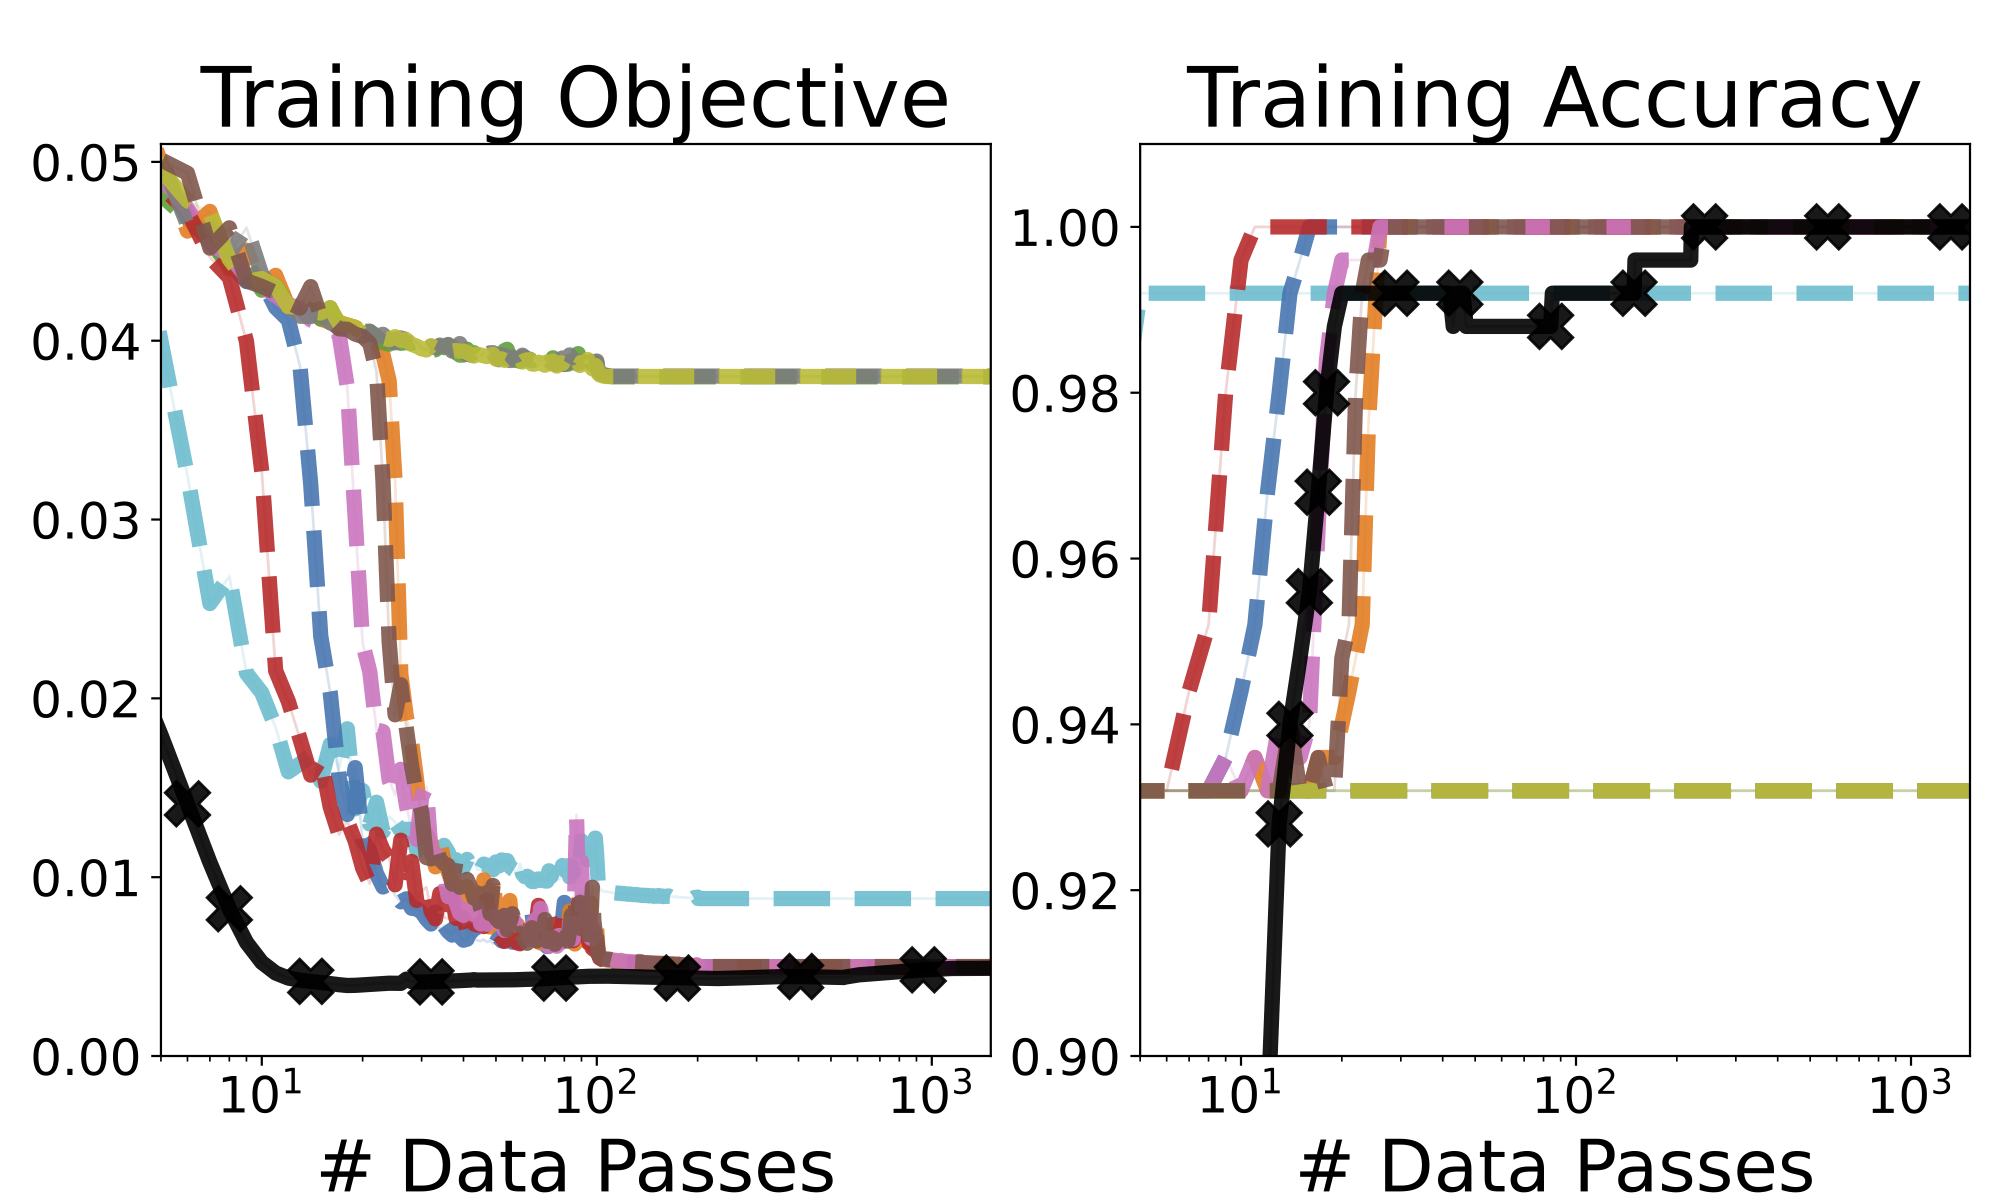
\includegraphics[width=.9\textwidth]{assets/synthetic_classification.png}
					\caption{Effect of random seed on convergence of SGD for a realizable problem.}
					\vspace{-1em}
					\label{fig:synthetic_classification}
				\end{figure}

			\end{block}

			\begin{block}{Convex Reformulations: ReLU Networks}

				\begin{columns}[t]
					\begin{column}{0.62\textwidth}

						\large
						{\Large \red{Non-Convex Problem}:}
						\vspace{1em}
						\[
							\Large
							\min_{w^1, w^2} \underbrace{\norm{\sum_{j=1}^m (X w^1_j)_+ w_j^2 - y}_2^2}_{\text{Squared Error}}
							+ \underbrace{\lambda \sum_{j=1}^m \norm{w^1_j}_2^2 + \norm{w^2_j}_2^2}_{\text{Weight Decay}},
						\]
						where \( \rbr{x}_+ = \max\cbr{x, 0} \) is the ReLU activation.


						\vspace{2.5em}
						\hrule
						\vspace{2.5em}

						{\Large \green{Convex Reformulation}}: {\normalsize \citep{pilanci2020convexnn}}
						\vspace{1em}
						\[ \Large
							\begin{aligned}
								\min_{v, h} & \norm{\sum_{j=1}^p D_j X (v_j - h_j) - y}_2^2 +
								\lambda \sum_{j=1}^p \norm{v_j}_2 + \norm{h_j}_2              \\
								            & \hspace{0.2em} \purple{\text{s.t. }
									v_j, h_j \in \calK_j := \cbr{w : (2D_j - I) X w \geq 0}},
							\end{aligned}
						\]

						\vspace{1em}
						where \( D_j = \text{diag}[\mathbbm{1}(X g_j \geq 0)] \).

					\end{column}

					\begin{column}{0.55\textwidth}
						\vspace{-2em}

						\begin{figure}[]
							\centering
							\begin{tikzpicture}[scale=2.5,
	]
	\begin{axis}[width=0.4\linewidth, height=8cm,
			axis lines=none,  % don't print axis lines
			yticklabels={,,}, xticklabels={,,},
			ymin=0, ymax=8, y axis line style={-},
			xmin=0, xmax=15, x axis line style={-},
		]
		\node [] (input) at (axis cs:0.5,4) {$X$};
		\node [Input] (input1) at (axis cs:3,2) {};
		\node [Input] (input2) at (axis cs:3,4) {};
		\node [Input] (input3) at (axis cs:3,6) {};

		\draw [decorate, line width = 0.6mm,
			decoration = {calligraphic brace}] (axis cs:1.5,1.5) --  (axis cs:1.5,6.5);

		\node [Hidden] (hidden1) at (axis cs:8,1) {};
		\node [Hidden] (hidden2) at (axis cs:8,3) {};
		\node [Hidden] (hidden3) at (axis cs:8,5) {};
		\node [Hidden] (hidden4) at (axis cs:8,7) {};

		\draw [->, style=arrow, draw=black] (input1) -- (hidden1);
		\draw [->, style=arrow, draw=black] (input2) -- (hidden1);
		\draw [->, style=arrow, draw=black] (input3) -- (hidden1);

		\draw [->, style=arrow, draw=black] (input1) -- (hidden2);
		\draw [->, style=arrow, draw=black] (input2) -- (hidden2);
		\draw [->, style=arrow, draw=black] (input3) -- (hidden2);

		\draw [->, style=arrow, draw=black] (input1) -- (hidden3);
		\draw [->, style=arrow, draw=black] (input2) -- (hidden3);
		\draw [->, style=arrow, draw=black] (input3) -- (hidden3);

		\draw [->, style=arrow, draw=red] (input1) -- (hidden4);
		\draw [->, style=arrow, draw=red] (input2) -- (hidden4);
		\draw [->, style=arrow, draw=red] (input3) -- (hidden4) node[pos=0.5,above] {$w^1_{j}$};

		\node [Output] (output) at (axis cs:13,4) {$\hat y$};

		\draw [->, style=arrow, draw=black] (hidden1) -- (output);
		\draw [->, style=arrow, draw=black] (hidden2) -- (output);
		\draw [->, style=arrow, draw=black] (hidden3) -- (output);
        \draw [->, style=arrow, draw=red] (hidden4) -- (output) node[pos=0.5,above] {$w^2_{j}$};
	\end{axis}

\end{tikzpicture}%

%\begin{tikzpicture}[scale=1,
%    ]
%    \begin{axis}[width=1.1\linewidth, height=5cm,
%            axis lines=none,  % don't print axis lines
%            yticklabels={,,}, xticklabels={,,},
%            ymin=-0.2, ymax=10.2, x axis line style={-},
%            xmin=-0.2, xmax=20.2, y axis line style={-},
%        ]

%        \filldraw[color=blue!60, fill=blue!5, line width=0.4mm](axis cs:0,5.8) rectangle (axis cs:20, 10);
%        \filldraw[color=red!60, fill=red!5, line width=0.4mm](axis cs:0,0) rectangle (axis cs:20, 4.2);

%        % non-convex models
%        \filldraw[line width=0.4mm, fill=white](axis cs:1,1) rectangle (axis cs:8, 3.2) node[pos=.5] {NC-GReLU};
%        \filldraw[line width=0.4mm, fill=white](axis cs:12,1) rectangle (axis cs:19, 3.2) node[pos=.5] {NC-ReLU};

%        % convex models
%        \filldraw[line width=0.4mm, fill=white](axis cs:1,6.8) rectangle (axis cs:8, 9) node[pos=.5] {C-GReLU};
%        \filldraw[line width=0.4mm, fill=white](axis cs:12,6.8) rectangle (axis cs:19, 9) node[pos=.5] {C-ReLU};

%        \draw [<->, solid, draw=black, line width = 0.6mm] (axis cs:4.5,3.2) -- (axis cs:4.5,6.8) node[right, pos=0.5] {\small Sol. Map};

%        \draw [<->, solid, draw=black, line width = 0.6mm] (axis cs:15.5,3.2) -- (axis cs:15.5,6.8)  node[right, pos=0.5] {\small Sol. Map};

%        \draw [<-, solid, draw=black, line width = 0.6mm] (axis cs:6,9) -- [bend left=15] (axis cs:14, 9);

%        \draw [->, solid, draw=orange, line width = 0.6mm] (axis cs:8,7.9) -- (axis cs:12,7.9);
%        \node[align=center] at (axis cs:10.1, 7.8) {\small Cone\\ \small Decomp.};
%    \end{axis}

%\end{tikzpicture}%


						\end{figure}

						\vspace{-3em}
						\begin{figure}[]
							\centering
							\begin{tikzpicture}[scale=2.5,
	]
	\begin{axis}[width=0.4\linewidth, height=8cm,
			axis lines=none,  % don't print axis lines
			yticklabels={,,}, xticklabels={,,},
			ymin=0, ymax=8, y axis line style={-},
			xmin=0, xmax=15, x axis line style={-},
		]
		\node [] (input1) at (axis cs:3,1) {$X$};
		\node [] (input2) at (axis cs:3,2.75) {$X$};
		\node [] (input3) at (axis cs:3,4.5) {$X$};

		\node [Splits] (hidden1) at (axis cs:9,1) {\scriptsize $D_3 X$};
		\node [Splits] (hidden2) at (axis cs:9,2.75) {\scriptsize $D_2 X$};
		\node [Splits] (hidden3) at (axis cs:9,4.5) {\scriptsize $D_1 X$};

		\draw [->, style=arrow, draw=black] (input1) -- (hidden1);

		\draw [->, style=arrow, draw=black] (input2) -- (hidden2);

		\draw [->, style=arrow, draw=red] (input3) -- (hidden3);

		\node [Output] (output) at (axis cs:13,2.75) {$\hat y$};

		\draw [->, style=arrow, draw=black] (hidden1) -- (output);
		\draw [->, style=arrow, draw=black] (hidden2) -- (output);
		\draw [->, style=arrow, draw=red] (hidden3) -- (output) node[pos=0.8,above] {$v_j$};

		\draw [draw=black, line width=0.3mm, dashed] (axis cs:4.65, 4.75) -- (axis cs:6.,6.6);
		\draw [draw=black, line width=0.3mm, dashed] (axis cs:6.5, 4.4) -- (axis cs:8.8,5.65);

		\node [draw=black, minimum size=0.2cm, shape=circle, solid, line width=0.5mm] (examine) at (axis cs:5.5,4.5) {};
		\node [draw=black, minimum size=1.4cm, shape=circle, solid, line width=0.5mm] (closeup) at (axis cs:7.5,6.2) {};

		\node [fill=white, draw=gray, line width=0.5mm, inner sep=0.07cm, shape=circle] at (axis cs:7.9,6.85) {};
		\node [fill=white, draw=gray, line width=0.5mm, inner sep=0.07cm, shape=circle] at (axis cs:7.15,6.9) {};
		\node [fill=white, draw=gray, line width=0.5mm, inner sep=0.07cm, shape=circle] at (axis cs:7.2,6.5) {};
		\node [fill=white, draw=gray, line width=0.5mm, inner sep=0.07cm, shape=circle] at (axis cs:6.3,6.25) {};

		\draw [draw=blue, dashed, line width=0.6mm] (axis cs:6.05,5.7) -- (axis cs:8.65,6.75);

		\node [fill=red, inner sep=0.08cm, shape=circle] at (axis cs:7.1,5.65) {};
		\node [fill=red, inner sep=0.08cm, shape=circle] at (axis cs:7.6,6.0) {};
		\node [fill=red, inner sep=0.08cm, shape=circle] at (axis cs:8.0,5.7) {};

	\end{axis}

\end{tikzpicture}%

%\begin{tikzpicture}[scale=1,
%    ]
%    \begin{axis}[width=1.1\linewidth, height=5cm,
%            axis lines=none,  % don't print axis lines
%            yticklabels={,,}, xticklabels={,,},
%            ymin=-0.2, ymax=10.2, x axis line style={-},
%            xmin=-0.2, xmax=20.2, y axis line style={-},
%        ]

%        \filldraw[color=blue!60, fill=blue!5, line width=0.4mm](axis cs:0,5.8) rectangle (axis cs:20, 10);
%        \filldraw[color=red!60, fill=red!5, line width=0.4mm](axis cs:0,0) rectangle (axis cs:20, 4.2);

%        % non-convex models
%        \filldraw[line width=0.4mm, fill=white](axis cs:1,1) rectangle (axis cs:8, 3.2) node[pos=.5] {NC-GReLU};
%        \filldraw[line width=0.4mm, fill=white](axis cs:12,1) rectangle (axis cs:19, 3.2) node[pos=.5] {NC-ReLU};

%        % convex models
%        \filldraw[line width=0.4mm, fill=white](axis cs:1,6.8) rectangle (axis cs:8, 9) node[pos=.5] {C-GReLU};
%        \filldraw[line width=0.4mm, fill=white](axis cs:12,6.8) rectangle (axis cs:19, 9) node[pos=.5] {C-ReLU};

%        \draw [<->, solid, draw=black, line width = 0.6mm] (axis cs:4.5,3.2) -- (axis cs:4.5,6.8) node[right, pos=0.5] {\small Sol. Map};

%        \draw [<->, solid, draw=black, line width = 0.6mm] (axis cs:15.5,3.2) -- (axis cs:15.5,6.8)  node[right, pos=0.5] {\small Sol. Map};

%        \draw [<-, solid, draw=black, line width = 0.6mm] (axis cs:6,9) -- [bend left=15] (axis cs:14, 9);

%        \draw [->, solid, draw=orange, line width = 0.6mm] (axis cs:8,7.9) -- (axis cs:12,7.9);
%        \node[align=center] at (axis cs:10.1, 7.8) {\small Cone\\ \small Decomp.};
%    \end{axis}

%\end{tikzpicture}%


						\end{figure}

					\end{column}

				\end{columns}

			\end{block}


		\end{column}

		\separatorcolumn

		\begin{column}{\colwidth}

			\vspace{-1.5em}
			\begin{block}{Problem Scale}
				\large

				The \textbf{convex program} enumerates all activation patterns,
				\vspace{0.5em}
				\[
					p = \abs{\cbr{D_j = \text{diag}[\mathbbm{1}(X g_j \geq 0)] : g_j \in \R^d }}.
				\]
				\vspace{-1em}
				\begin{itemize}
					\item \red{Exponential in general}: \( p \in O(r \cdot (\frac{n}{r})^r) \),
					      where \( r = \text{rank}(X) \) \citep{winder1966partitions}.
					      \begin{itemize}
						      \item \large But sub-sampling works well in practice.
					      \end{itemize}
					      \vspace{0.1em}

					\item \green{Highly structured} --- it's a huge-scale constrained generalized linear model!

					\item The convex reformulation \purple{exchanges one kind of hardness for another}.
				\end{itemize}
			\end{block}

			\vspace{-1em}
			\begin{block}{Gated ReLU Activations}
				\large

				\red{Issue}: convex problem is too large for IPMs, but projecting onto \( \calK_j \) is an LP.

				\green{Solution}: consider unconstrained relaxation:
				\[
					\begin{aligned}
						\textbf{C-GReLU}: \min_{u} & \norm{\sum_{j=1}^p D_j X u_j - y}_2^2 +
						\lambda \sum_{j=1}^p \norm{u_j}_2                                    \\
					\end{aligned}
				\]

				\begin{beamercolorbox}[wd=\textwidth,sep=1em]{result}
					\textbf{Theorem 2.2} (informal): C-GReLU is equivalent to solving
					\[
						\textbf{NC-GReLU}: \min_{w^1, w^2} \half \norm{\sum_{j=1}^p \phi_{g_j}(X, w^1_{j})w^2 - y}_2^2 + \frac{\lambda}{2} \sum_{j=1}^p \norm{w^1_{j}}_2^2 + \norm{w_j^2}_2^2,
					\]
					with the ``Gated ReLU'' \citep{fiat2019decoupling} activation function
					\[ \phi_{g}(X, u) = \text{diag}(\mathbbm{1}(Xg \geq 0)) X u, \]
					and gate vectors \( g_j \) such that \( D_j = \text{diag}[\mathbbm{1}(X g_j \geq 0) \).
				\end{beamercolorbox}

				\textbf{Interpretation}: if \( u_j \not \in \calK_j \), then activation
				must be decoupled from weights.

			\end{block}
			\vspace{-1em}
			\begin{block}{Cone Decompositions}
				\large
				{ \Large
					\red{Q}: when are Gated ReLU and ReLU networks equivalent?

					\green{A}: if we can decompose \( u_j = v_j - h_j \) for some \( v_j, h_j \in \calK_j \).
				}

				\begin{figure}[t]
					%! TEX root = ../../main.tex

%% Illustration of cone decomposition. 

\begin{tikzpicture}[scale=1,
		declare function={
				cone_u(\x)= -\x/3;
				cone_l(\x)= -4*\x/5;
			}
	]
	\begin{axis}[width=0.9\linewidth, height=14cm,
			axis lines=center, yticklabels={,,}, xticklabels={,,},
			ymin=-4, ymax=4, ytick={-5,...,5}, ylabel=$$, x axis line style={-},
				xmin=-6, xmax=6, xtick={-5,...,5}, xlabel=$$, y axis line style={-},
		]
		\addplot[name path=cone_u, domain=-6:6, samples=100, line width=6pt]{cone_u(x)};
		\addplot[name path=cone_l, domain=-6:6, samples=200, line width=6pt]{cone_l(x)};

		% add color fill to both cones.
		\addplot fill between[
				of = cone_u and cone_l,
				split, % calculate segments
				every even segment/.style = {fill=blue, fill opacity=0.3},
				every odd segment/.style  = {fill=teal, fill opacity=0.3}
			];

		%% point labels
		% origin point
		\node[circle, fill, inner sep=5pt] at (axis cs:0,0) {};

		\node[label={0:\Large $u_j$}, circle, fill, inner sep=8pt] (u) at (axis cs:2,1) {};
		\node[label={90:\Large $v_j$}, circle, fill, inner sep=8pt] (v) at (axis cs:25/7+2, -25/21 - 2/3) {};
		\node[label={90:\Large $w_j$}, circle, fill, inner sep=8pt] (w) at (axis cs:-25/7, 20/7) {};

		% labels
		\node[label={0:\huge$\calK_j$}] at (axis cs:4,-2.5) {};
        \node[label={180:\huge$-\calK_j$}] at (axis cs:-3.75,2.5) {};

		% lines
		\draw [->, dotted, draw=red, line width = 2.5mm] (u) edge (w);
		\draw [->, dotted, draw=red, line width = 2.5mm] (u) edge (v);
	\end{axis}

\end{tikzpicture}%

					\caption{Illustration of cone decomposition procedure.}
					\label{fig:cone-decomp}
				\end{figure}

				\textbf{Existence} of ``cone decompositions'':
				\vspace{-0.5em}
				\begin{itemize}
					\item We can guarantee \( \calK_j - \calK_j = \R^d \) if \( X \) is \green{full row-rank}.
					\item More generally, we show ``flat'' \( \calK_j \) can be \green{safely merged} into other neurons.
				\end{itemize}
			\end{block}
		\end{column}

		\separatorcolumn

		\begin{column}{\colwidth}
			\vspace{-1.5em}
			\begin{block}{Main Approximation Result}

				\large
				\vspace{1em}

				\begin{beamercolorbox}[wd=\textwidth,sep=1em]{result}
					\textbf{Theorem 3.7} (informal):
					Let \( \lambda \geq 0 \) and let \( p^* \) be the optimal value of the ReLU problem.
					There exists a C-GReLU problem with minimizer \( u^* \) and optimal value \( d^* \) satisfying,
					%\vspace{-1em}
					{ \Large
							\[
								d^* \leq p^* \leq d^* + \textcolor{Red}{2 \lambda \kappa(\tilde X_{\calJ}) \sum_{D_i \in \tilde \calD} \norm{u_i^*}_2}.
							\]
						}
				\end{beamercolorbox}
				\textbf{Consequence}: ReLU and Gated ReLU model classes are equivalent!

			\end{block}
			\vspace{-1em}
			\begin{block}{Algorithms}

				\large
				We develop two algorithms for solving the convex reformulations:
				\vspace{-0.5em}
				\begin{itemize}
					\item \textbf{R-FISTA}: a restarted FISTA variant for Gated ReLU.
					\item \textbf{AL}: an augmented Lagrangian method for the (constrained) ReLU Problem.
				\end{itemize}

				And we can use all the \green{convex tricks}!
				\vspace{-0.5em}
				\begin{itemize}
					\item \textbf{Fast}: \( O(1/t^2) \) convergence rate.

					\item \textbf{Tuning-free}: line-search, restarts, data normalization, \ldots

					\item \textbf{Certificates}: termination based on minimum-norm subgradient.
				\end{itemize}
			\end{block}
			\vspace{-1em}
			\begin{block}{Experiments}
				\large
				\begin{figure}[]
					\centering
					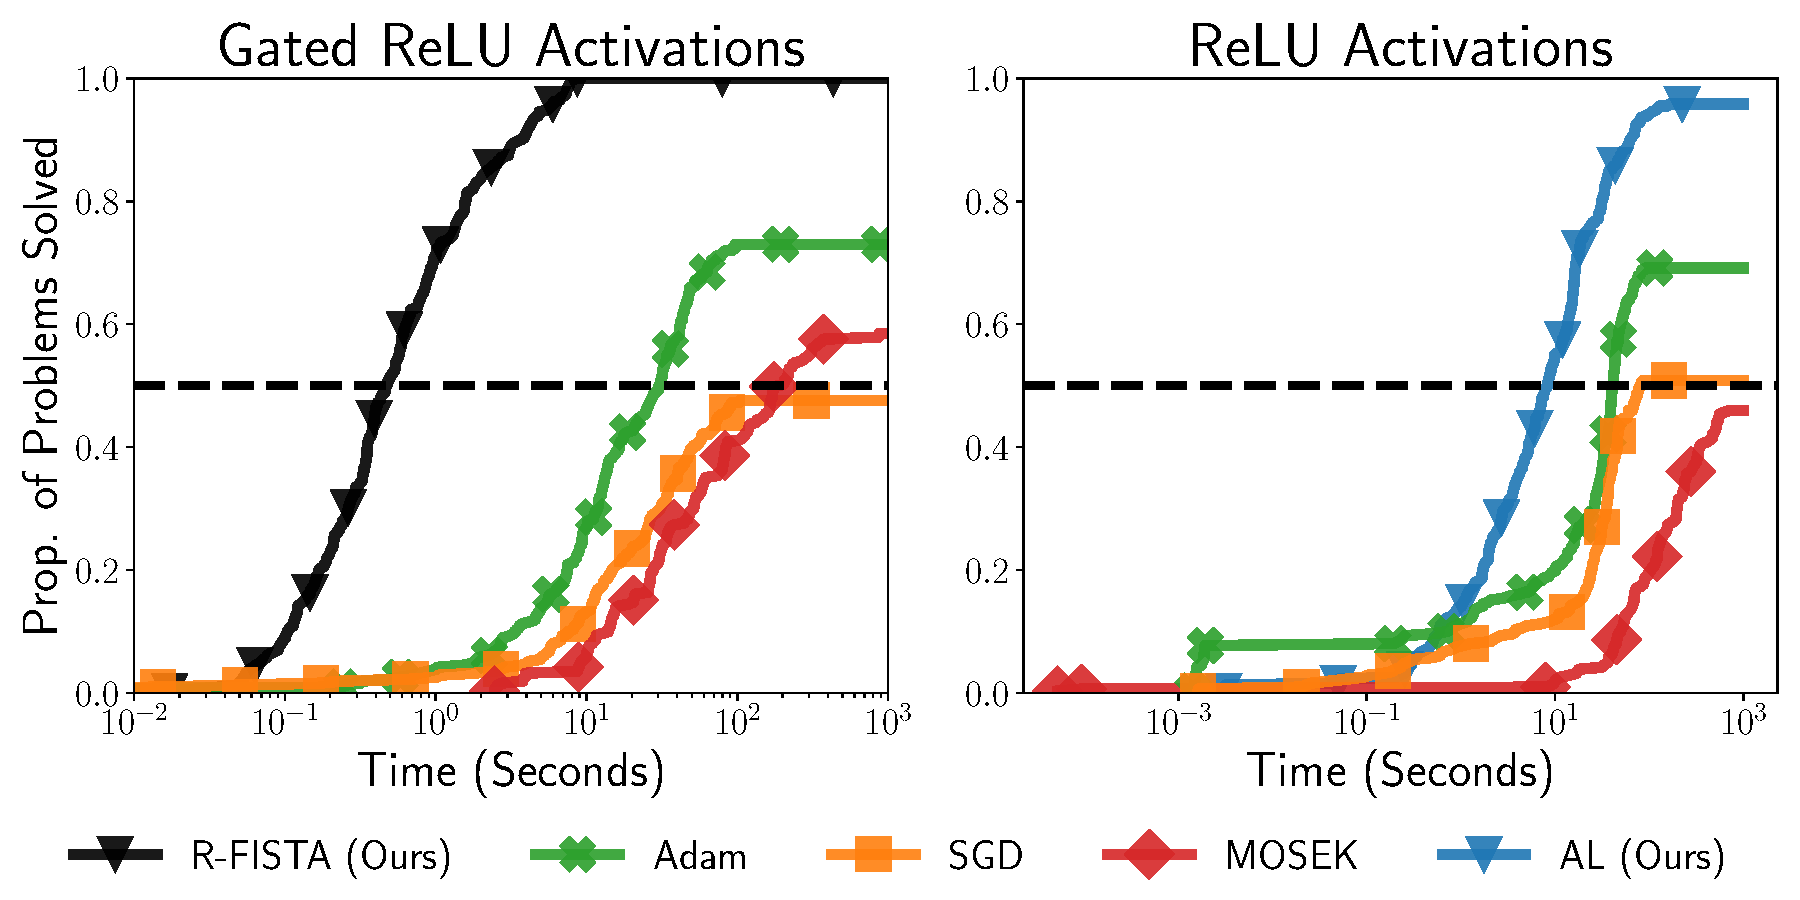
\includegraphics[width=\textwidth]{assets/pp_main.pdf}
					\caption{Performance profile comparing convex solvers to Adam and SGD.}
					\label{fig:performance-profile}
				\end{figure}
				\vspace{-0.5em}
				\begin{itemize}
					\item Performance on 438 training problems generated from the UCI repository.
					\item R-FISTA/AL solve \textbf{more problems, faster}, than SGD and Adam.
				\end{itemize}
			\end{block}
			\vspace{-1em}
			\begin{block}{References}

				\footnotesize{
					\bibliography{
						bib/monographs.bib,
						bib/gradient_methods.bib,
						bib/lower_bounds.bib,
						bib/assumptions.bib,
						bib/interpolation.bib,
						bib/step_sizes.bib,
						bib/datasets.bib,
						bib/general_refs.bib}
				}
				\bibliographystyle{icml2022}

			\end{block}

		\end{column}

		\separatorcolumn
	\end{columns}
\end{frame}

\end{document}
